\documentclass[letterpaper, 12pt]{article}
\usepackage{graphicx}
%This is the margin, it makes stuff look pretty but it's really not needed
\usepackage[margin=1in]{geometry}
%These packages are needed if you want to do some math stuff (I think)
\usepackage{amsmath}
\usepackage{amssymb}
%This package allows allows for headers and footers, which I think add to the look of the document
\usepackage{fancyhdr}

%The pagestyle calls from the fancyhdr package, but it can be set to a lot of other things without the package
\pagestyle{fancy}

%Gets rid of the default formatting when using the fancy pagestyle
\fancyhf{}
%Defining the header (by default, fancy includes a line on top and bot, I like it so I'm not getting rid of it!)
\rhead{
    Shengdong Li
    Table 7
    Calc 1
}
%Defining the footer
\rfoot{Page \thepage}

%The "body"/visible section of the tex file
\begin{document}
%Title page
\title{Response to Camden Maggard}
\author{by Shengdong Li}
\date{4 April 2020}
\maketitle

\section{Intro}
Hey Camden! Really good job on the initial post, I haven't even gone close to thinking about using the critical points of the graphs to prove that the two expressions are equal!
However, I would like to make a suggestion regarding the use of equation editors.

\section{Latex editors}
Originally, I thought that using the Canvas equation editor was slow too: going in and out of the editor was aggravating. In addition to this, the finished equations mixed in with the regular text often looked messy and unorganized. \\~\\
However, the alternative to this, using a latex editor, seemed very complicated. I was worried that it was going to be like learning a computer language, with brackets and parenthesis and commands and keyphrases that you had to memorize. \\~\\
But then a few days ago, thanks to an abundant amount of freetime, I finally sat down and tried to learn latex, and surprisingly, it was much easier than I thought. After just one or two 15 minute youtube videos I realized that it was much less complicated and hard to learn than I thought it would be. Addition, subtraction, and power are just \string+, \string-, and \string^ respectively, and learning other syntax, like sin and integrals are just 10 second google searches.
I would highly recommend you check out latex, if you have some spare time. Overleaf is a decent online latex editor.

\section{Uploading to Canvas}
By the way, did you know that you can embed many types of google drive files into canvas?\\~\\
First, open the doc on google drive.
\begin{center}
    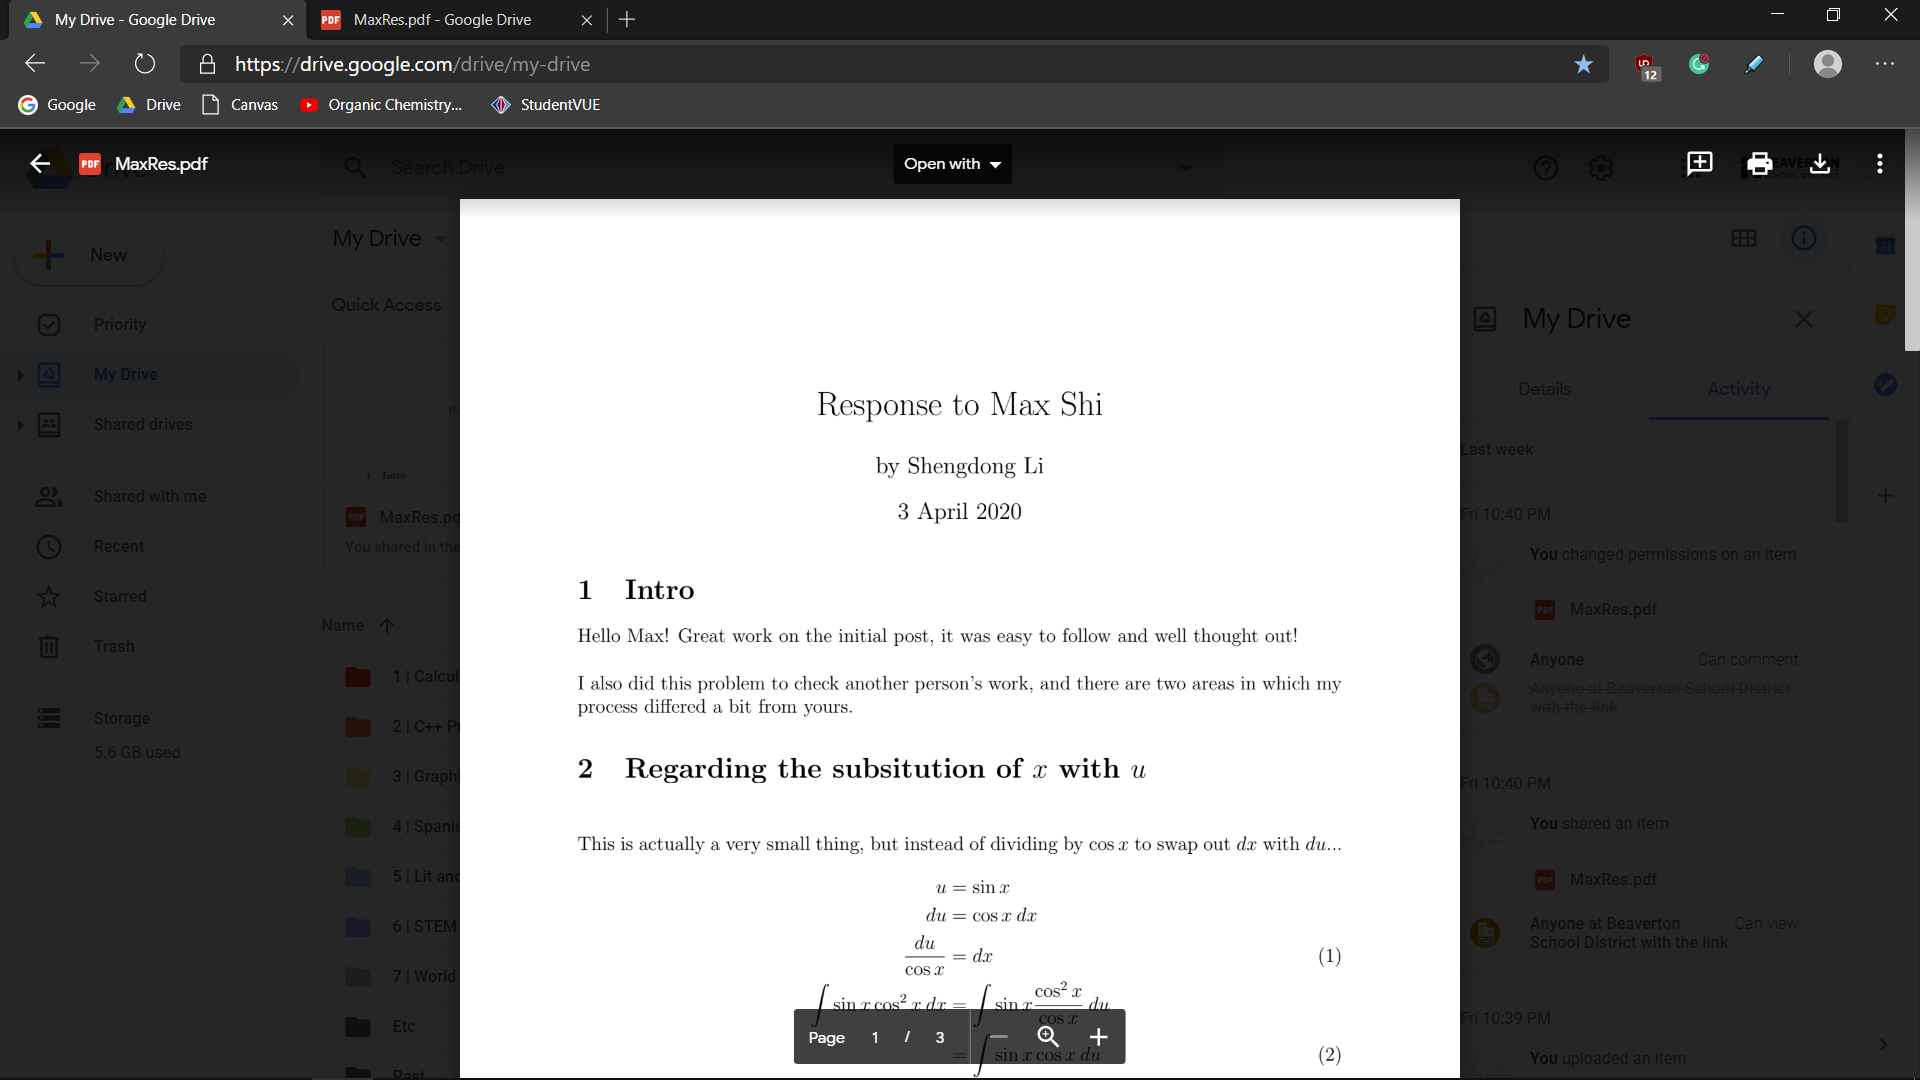
\includegraphics[scale=0.3]{1.png}
\end{center}
Then, click on the 3 dots on the top right, and click on open in new window
\begin{center}
    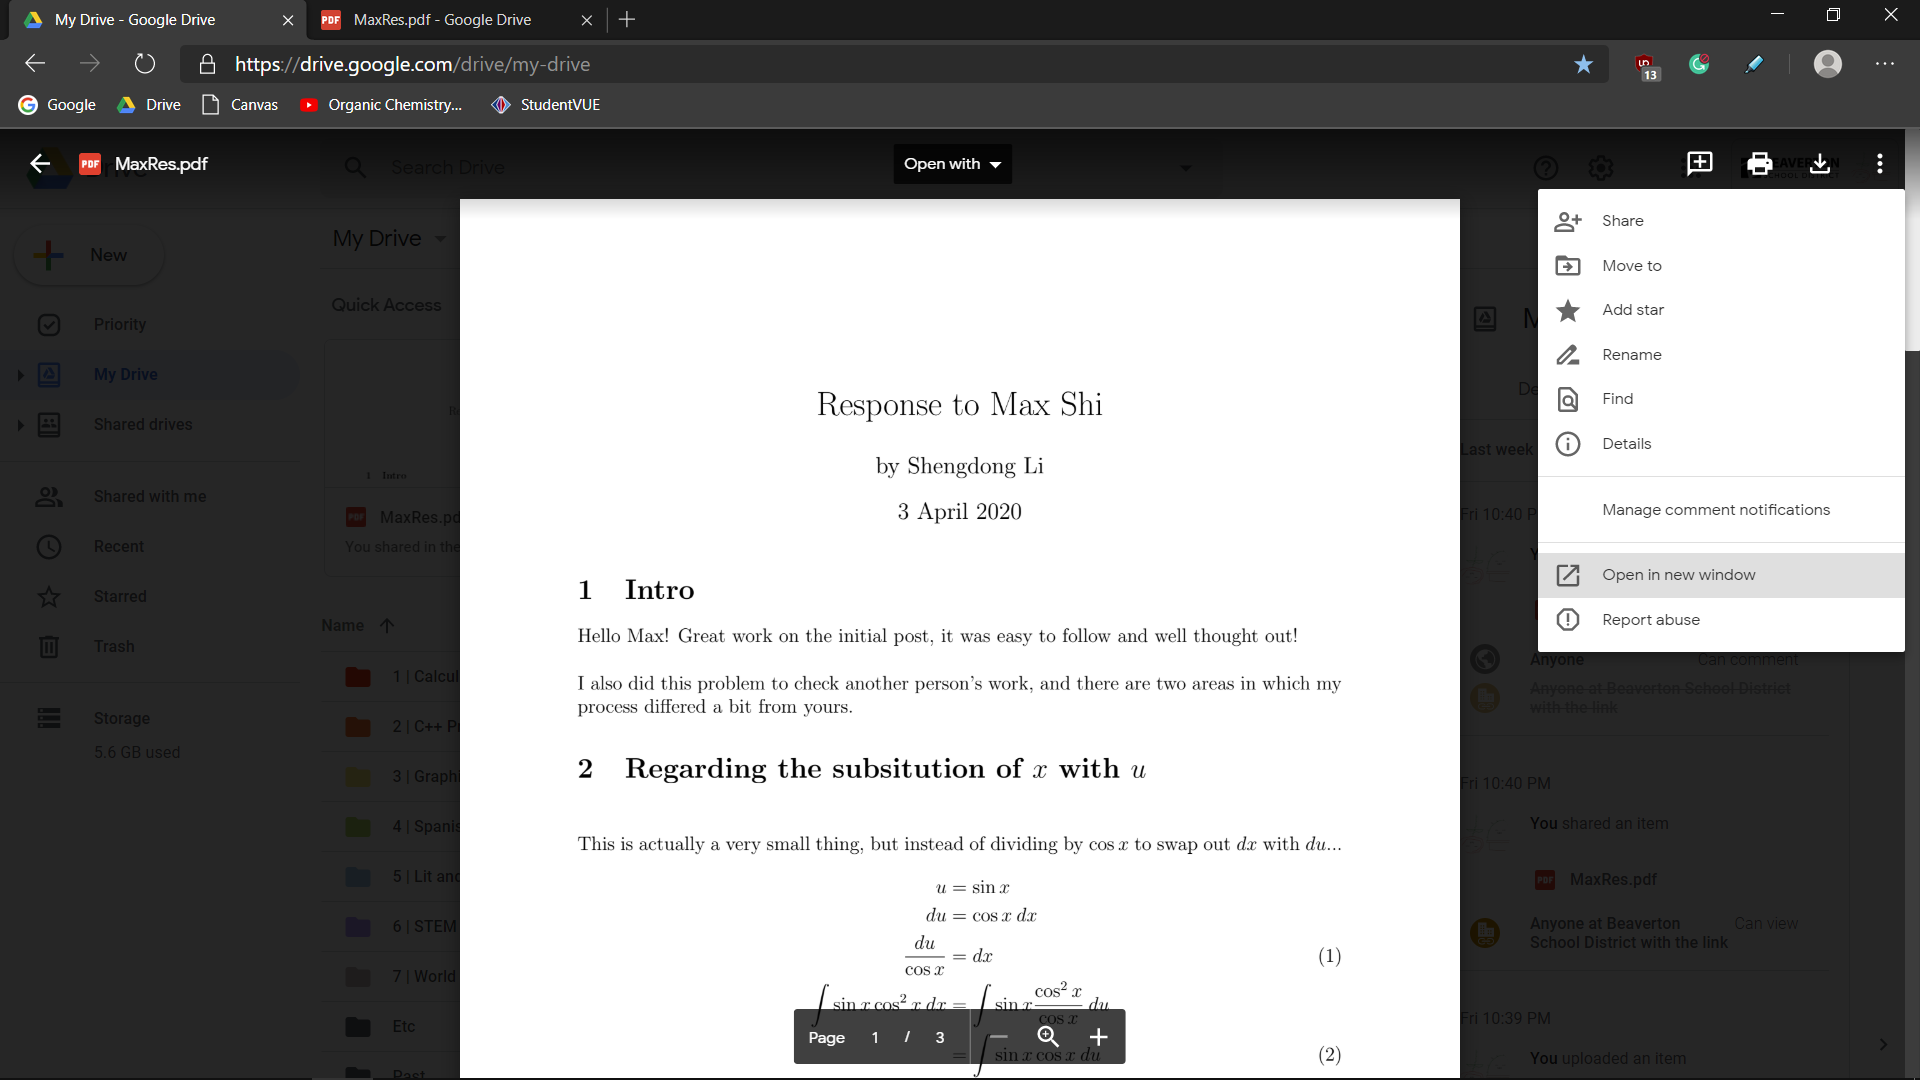
\includegraphics[scale=0.3]{2.png}
\end{center}
A new tab should pop up.
\begin{center}
    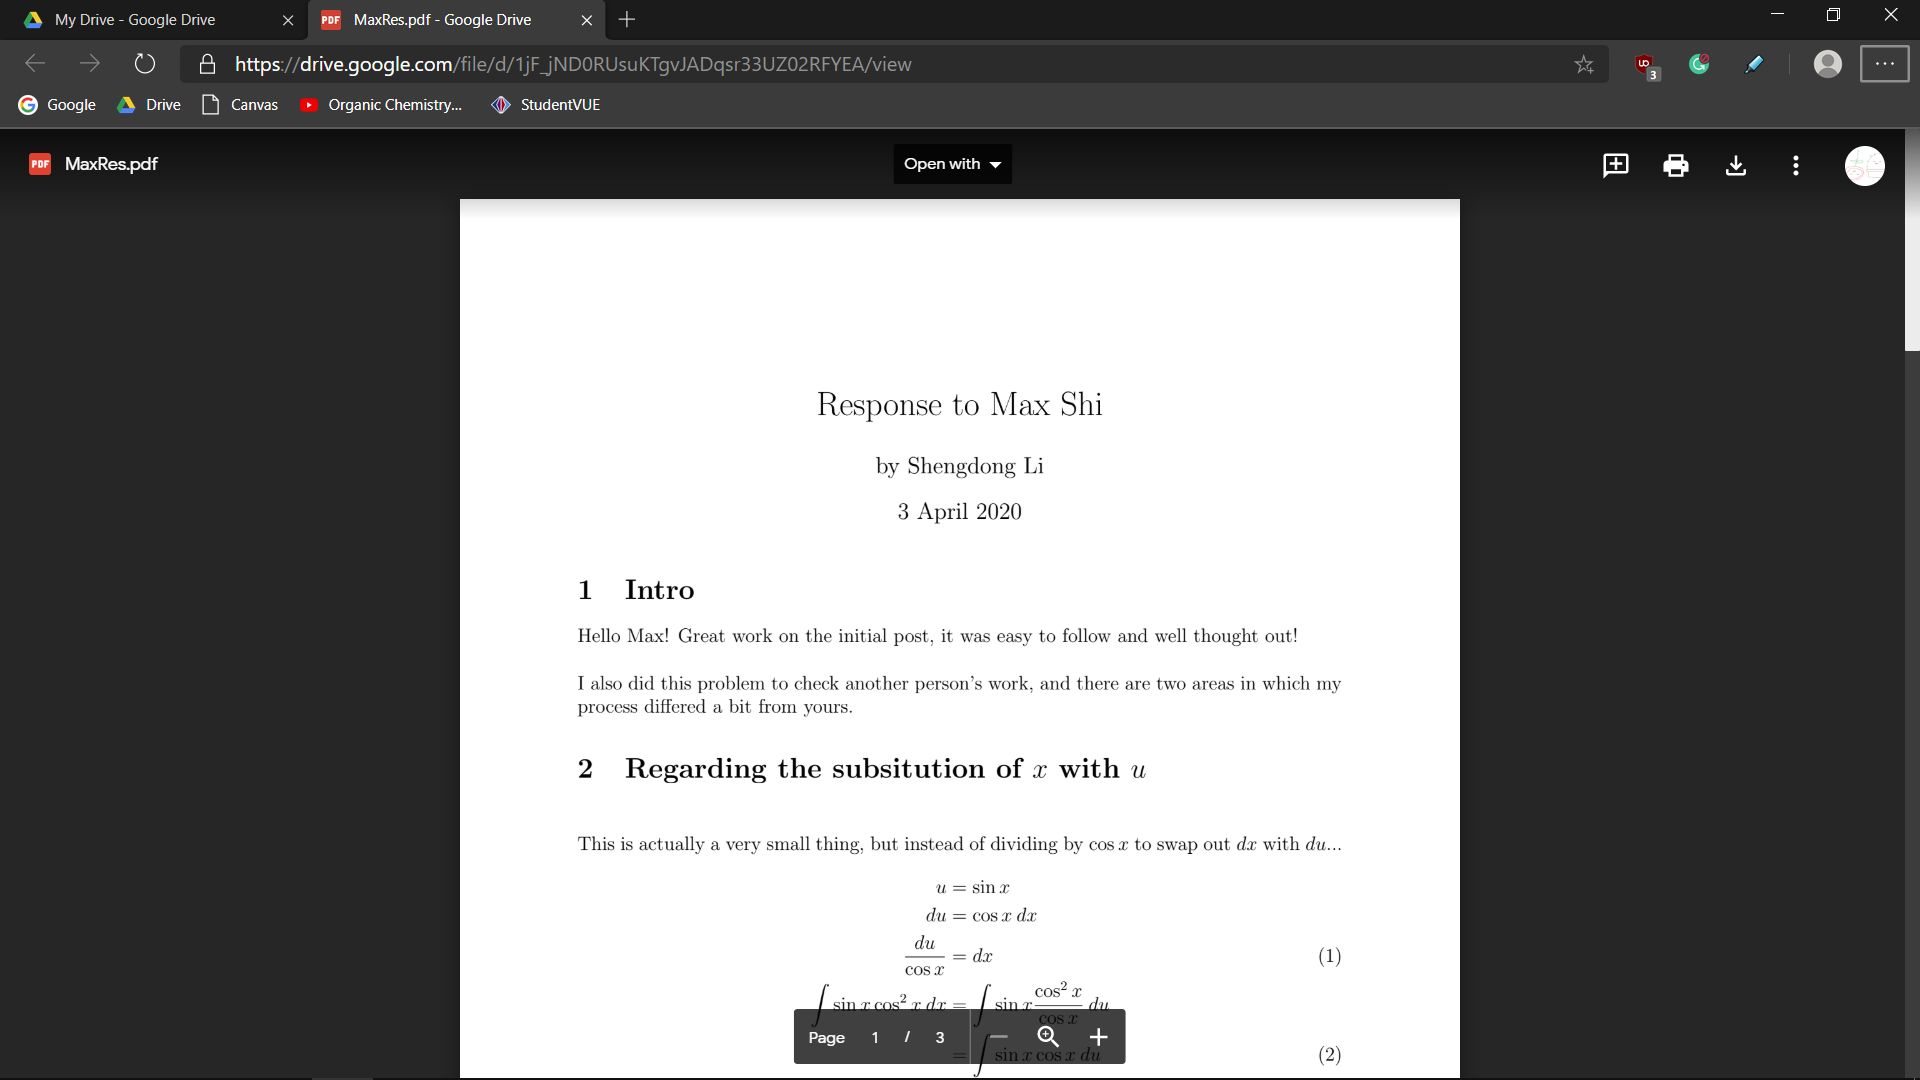
\includegraphics[scale=0.3]{3.png}
\end{center}
Click on the 3 dots on the top right again and then on embed item
\begin{center}
    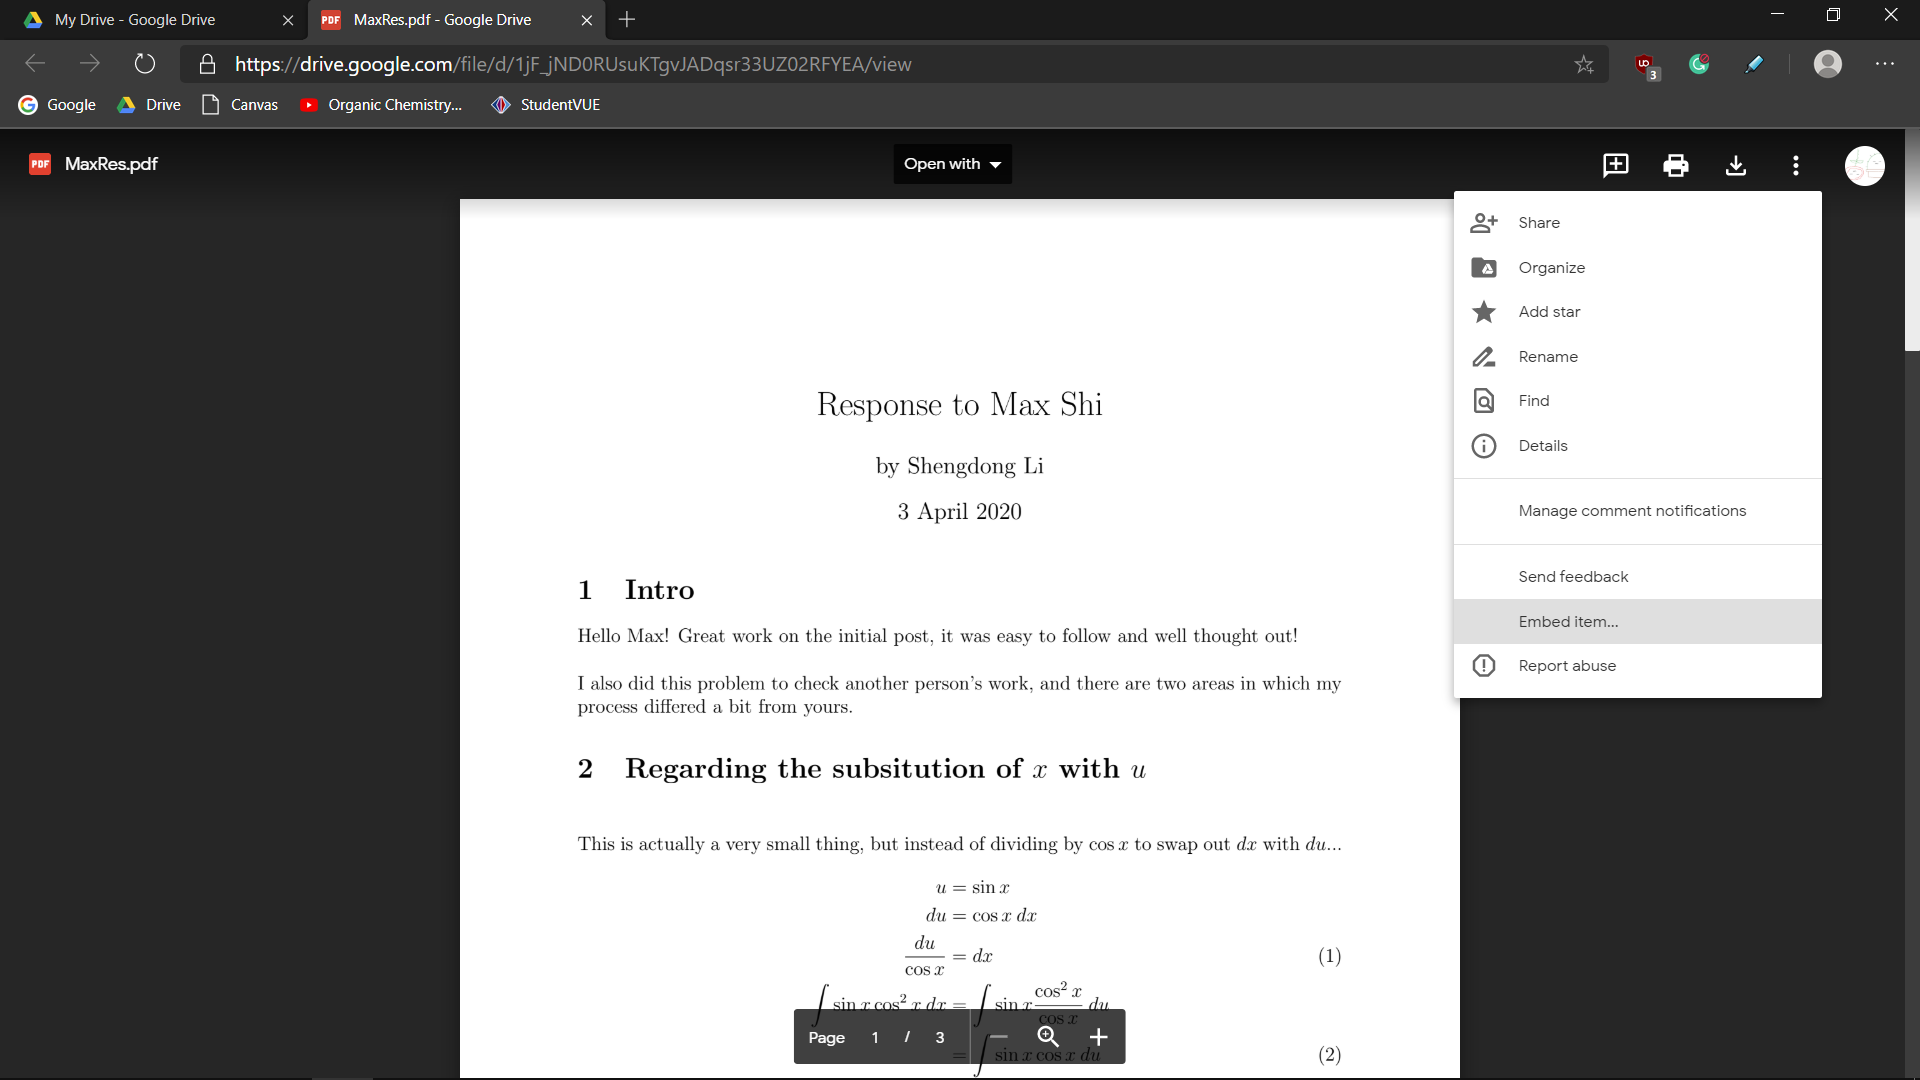
\includegraphics[scale=0.3]{4.png}
\end{center}
This box should pop up. Copy the text in there.
\begin{center}
    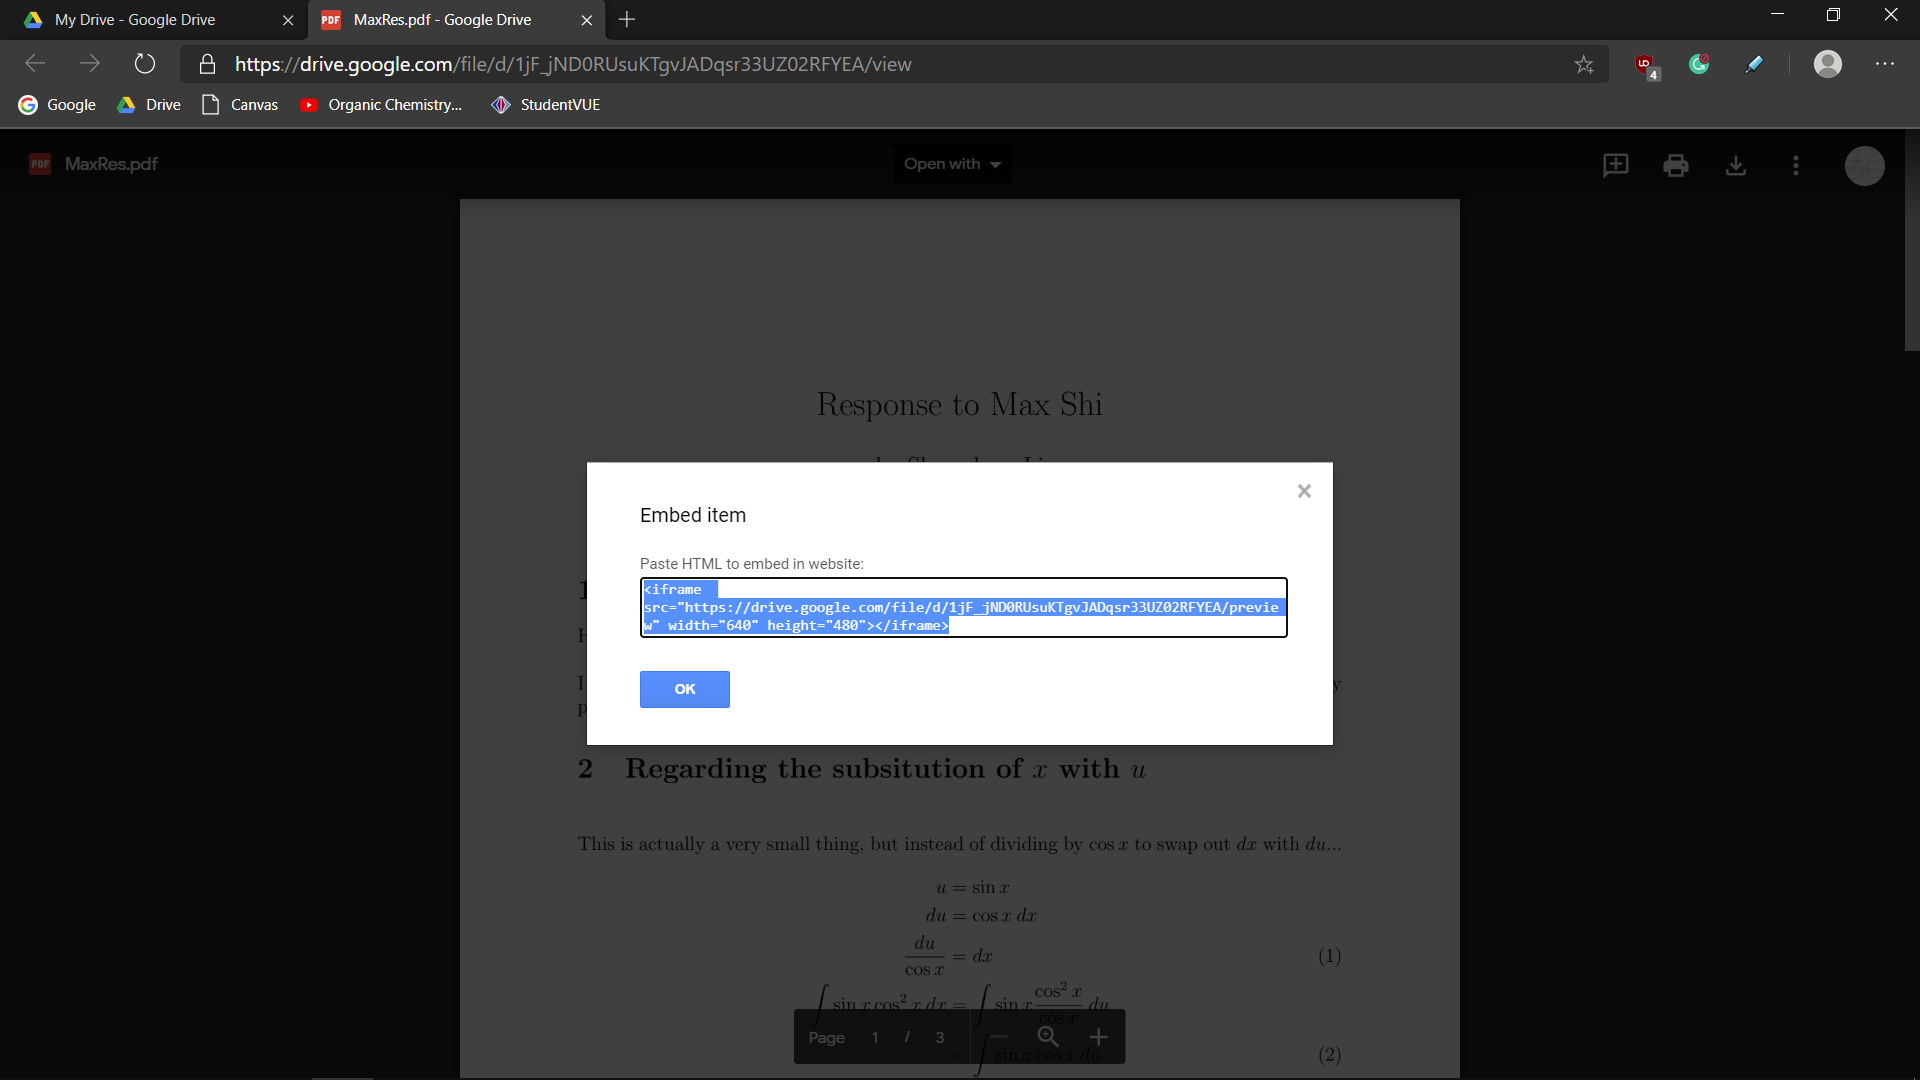
\includegraphics[scale=0.3]{5.png}
\end{center}
Then in Canvas, click on insert/edit media
\begin{center}
    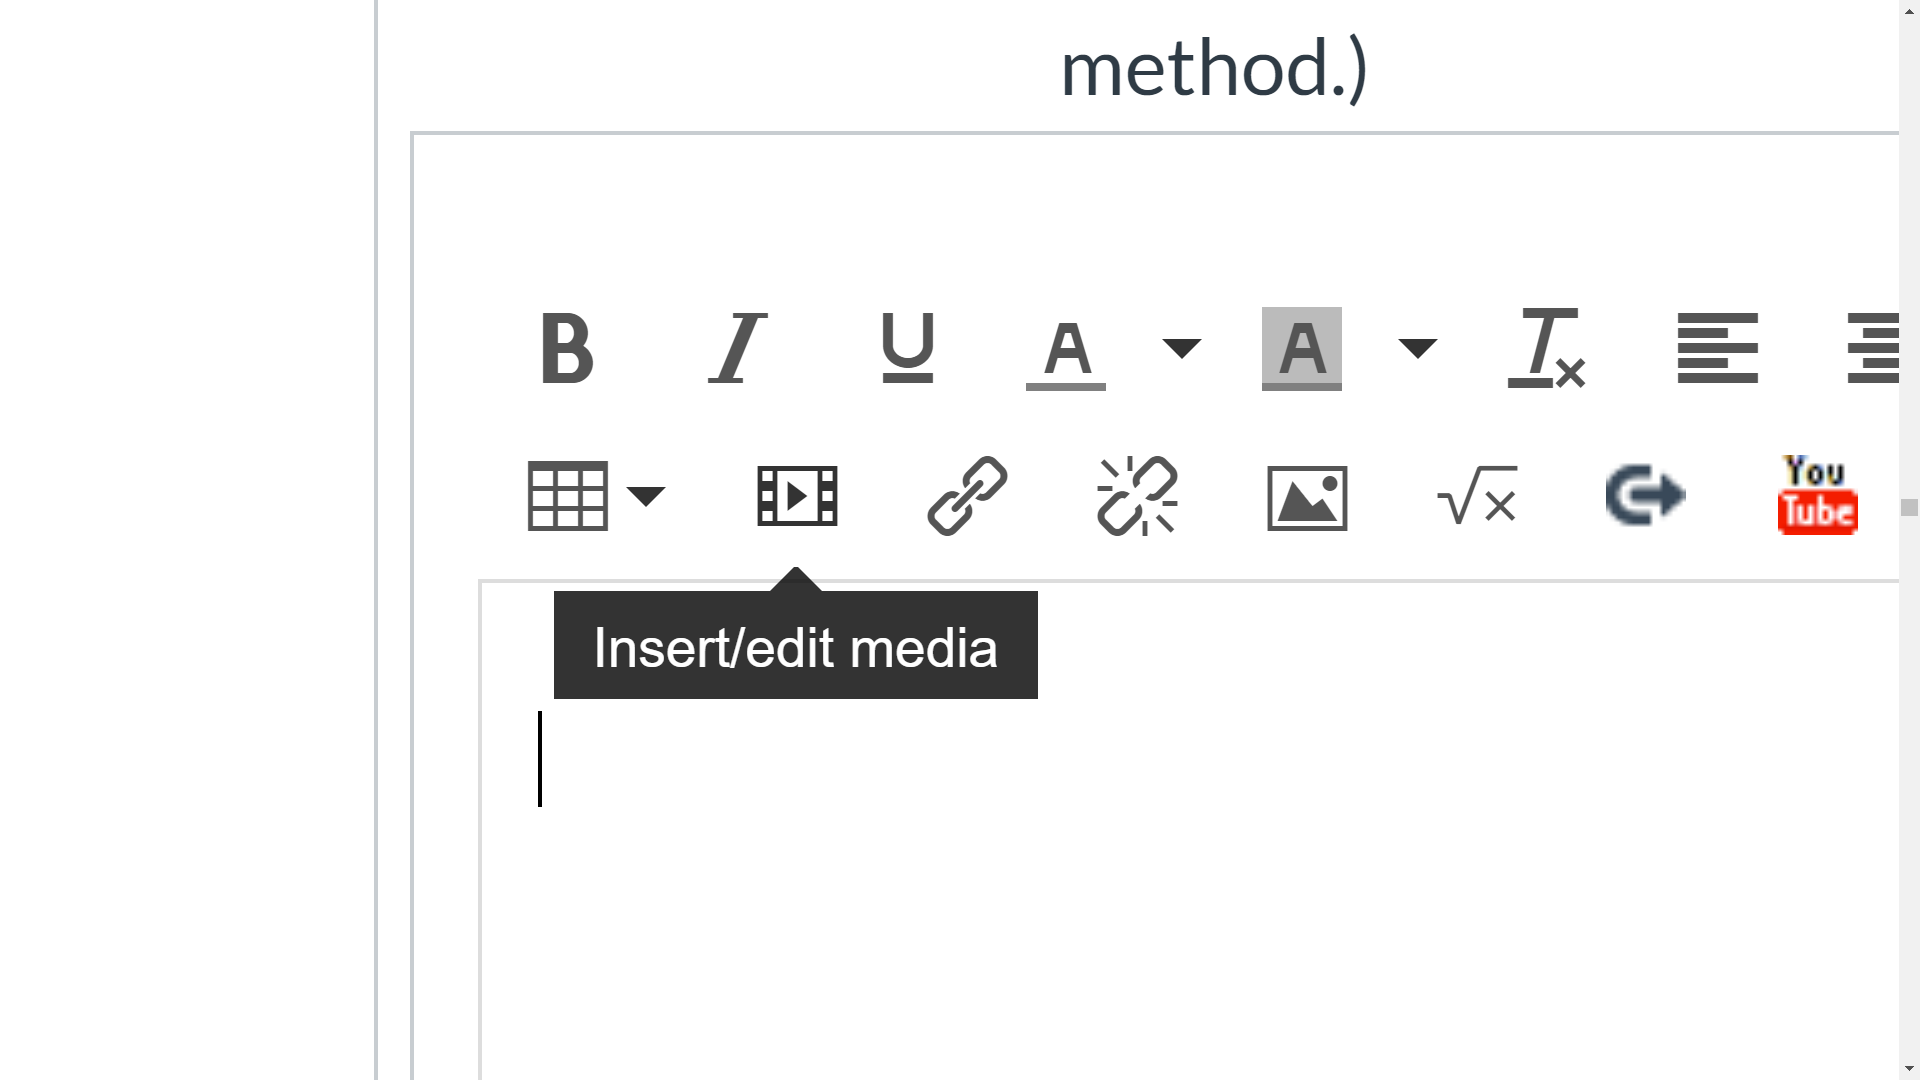
\includegraphics[scale=0.3]{6.png}
\end{center}
Open the embed tab, then copy and paste the embed code from earlier
\begin{center}
    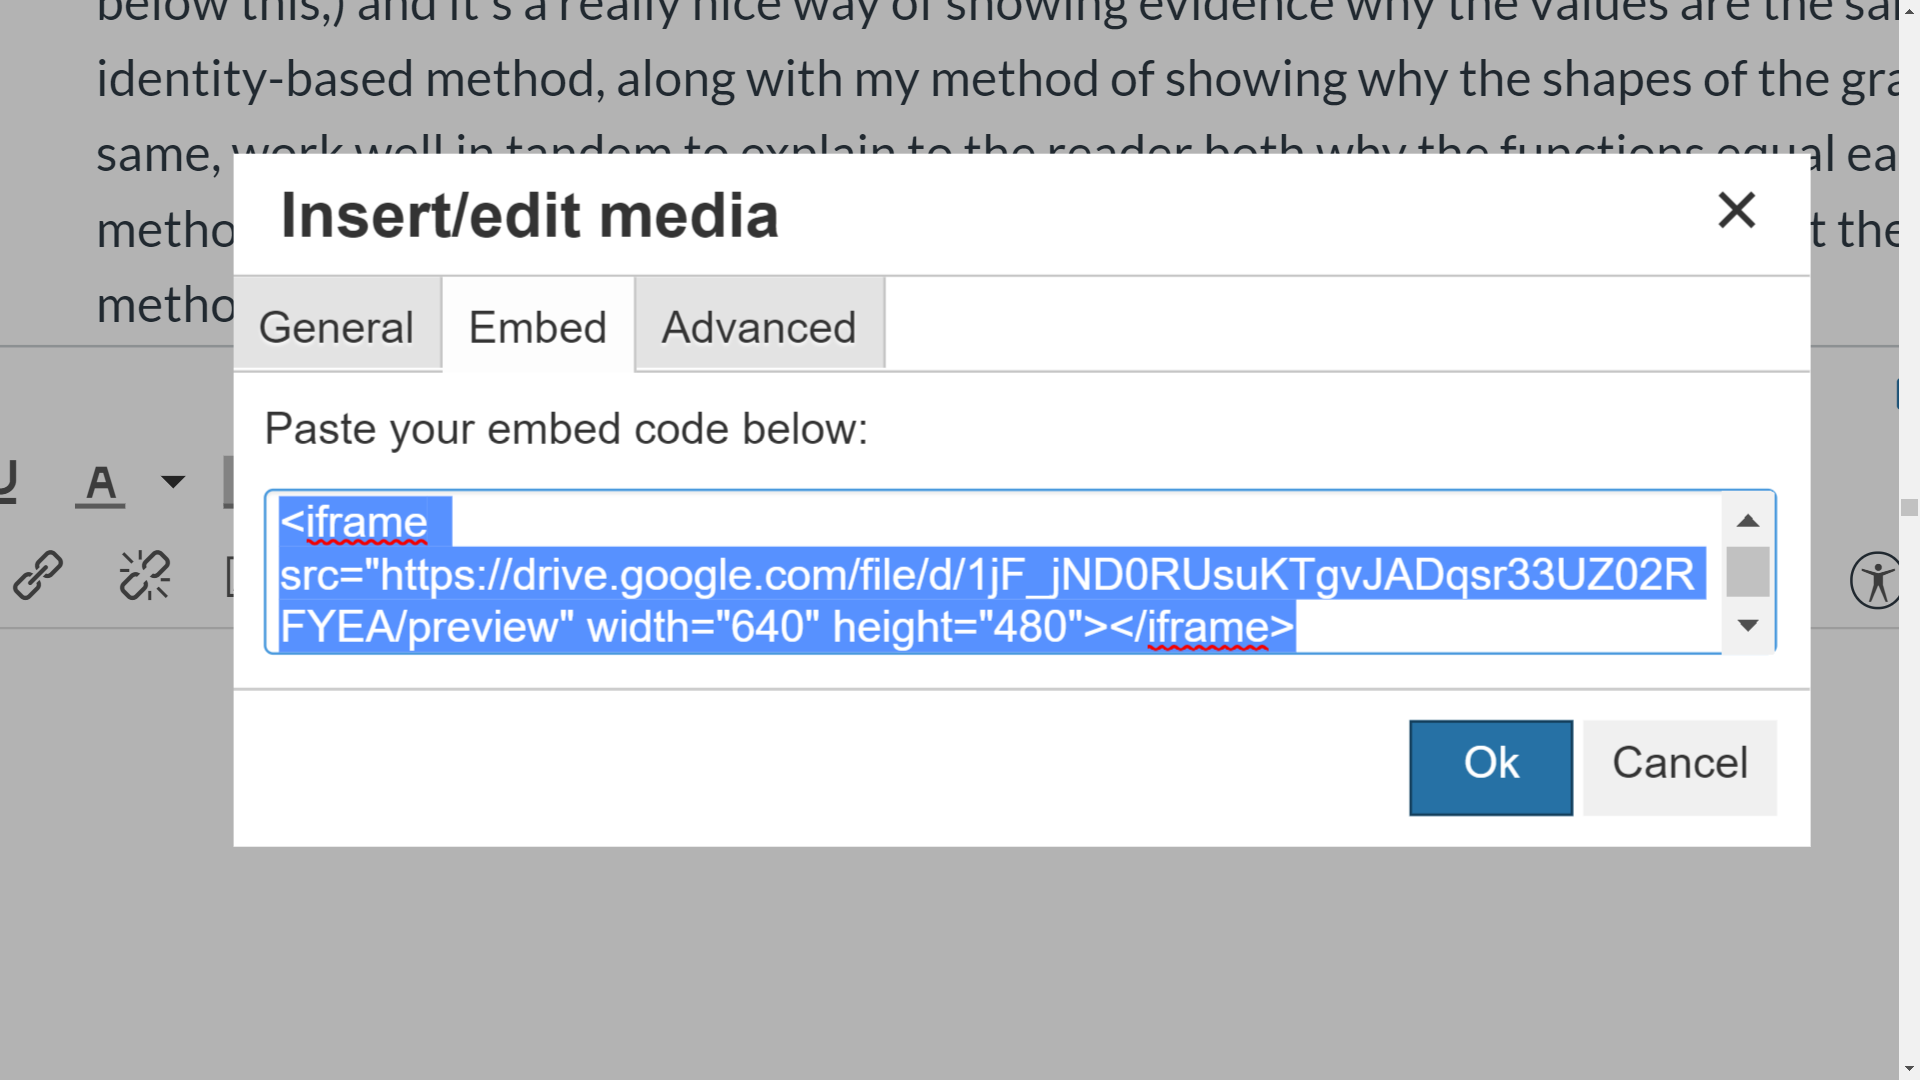
\includegraphics[scale=0.3]{7.png}
\end{center}
Click ok, and you should have an embedded item, like this:
\begin{center}
    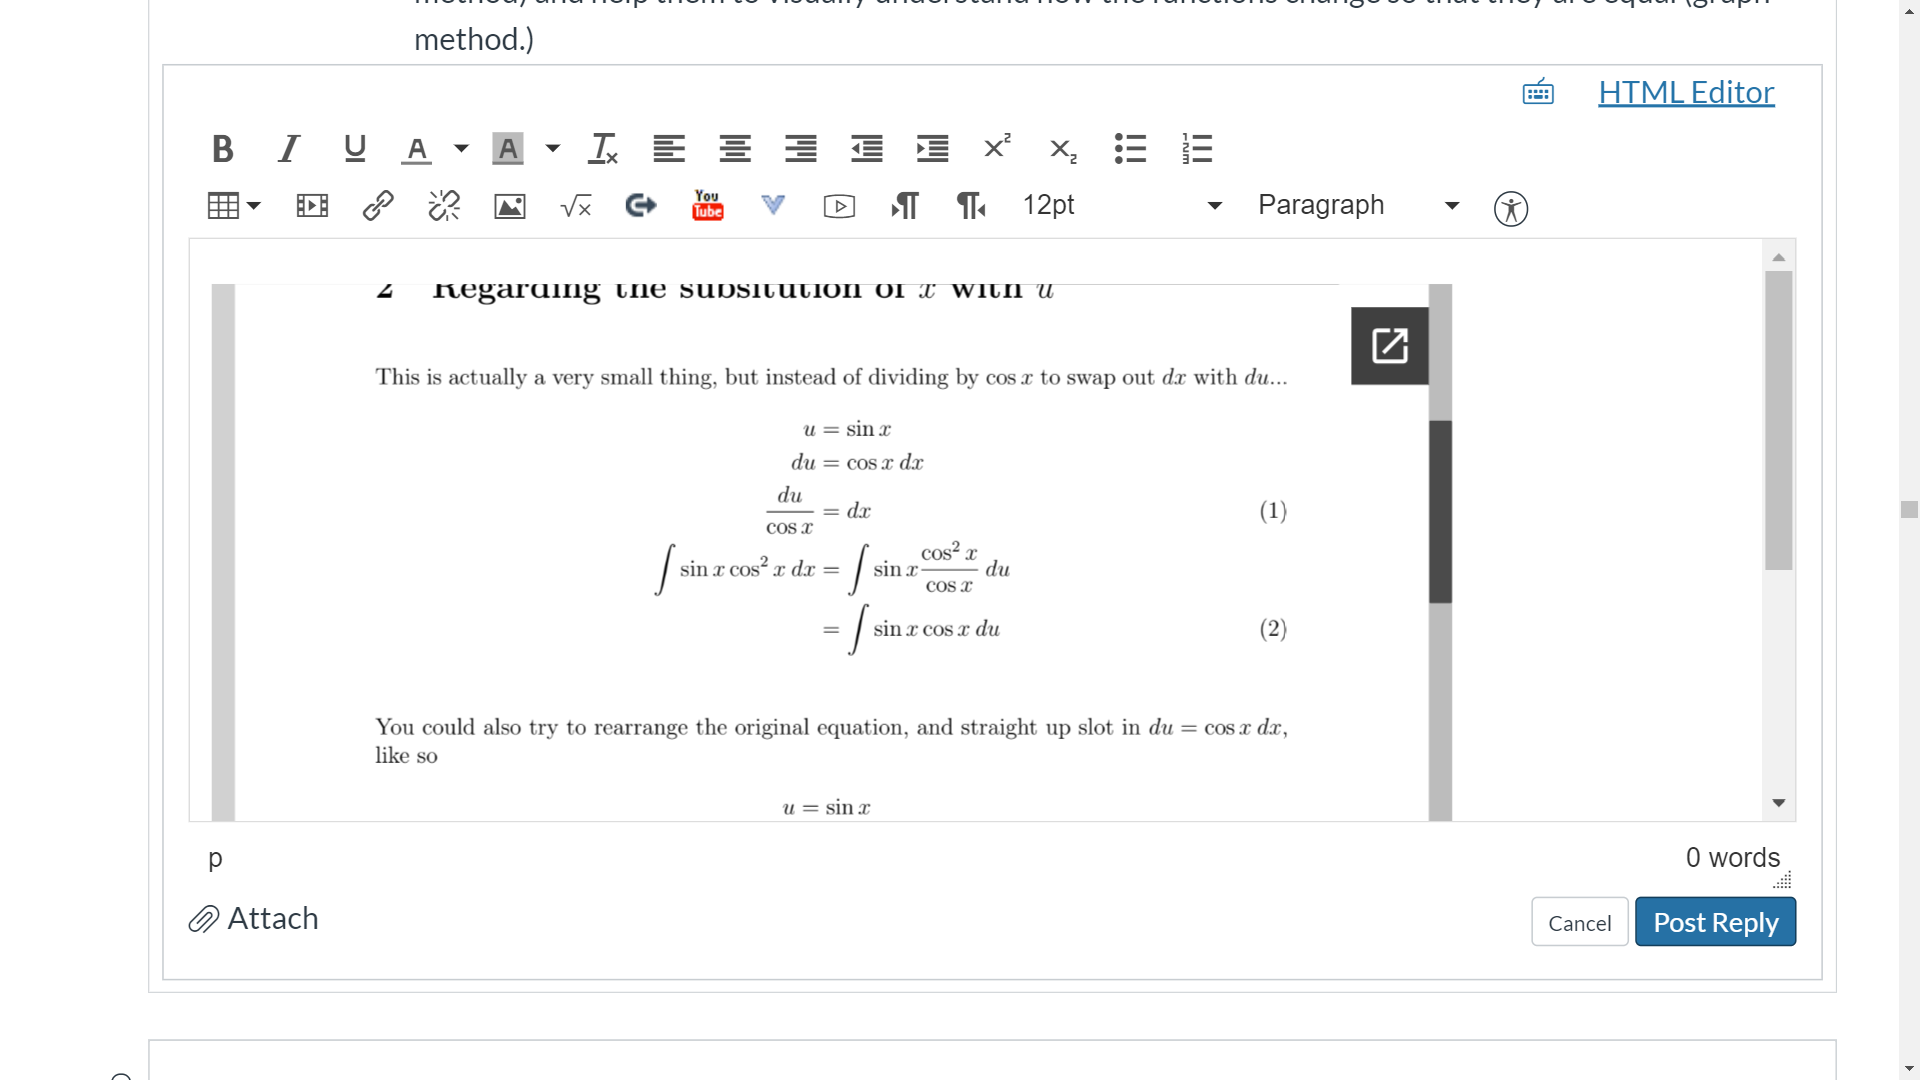
\includegraphics[scale=0.3]{8.png}
\end{center}
Keep in mind that you must change the sharing permissions on the document to something like "anyone at beaverton school district can find access" or other people will not be able to see your embedded file.
\begin{center}
    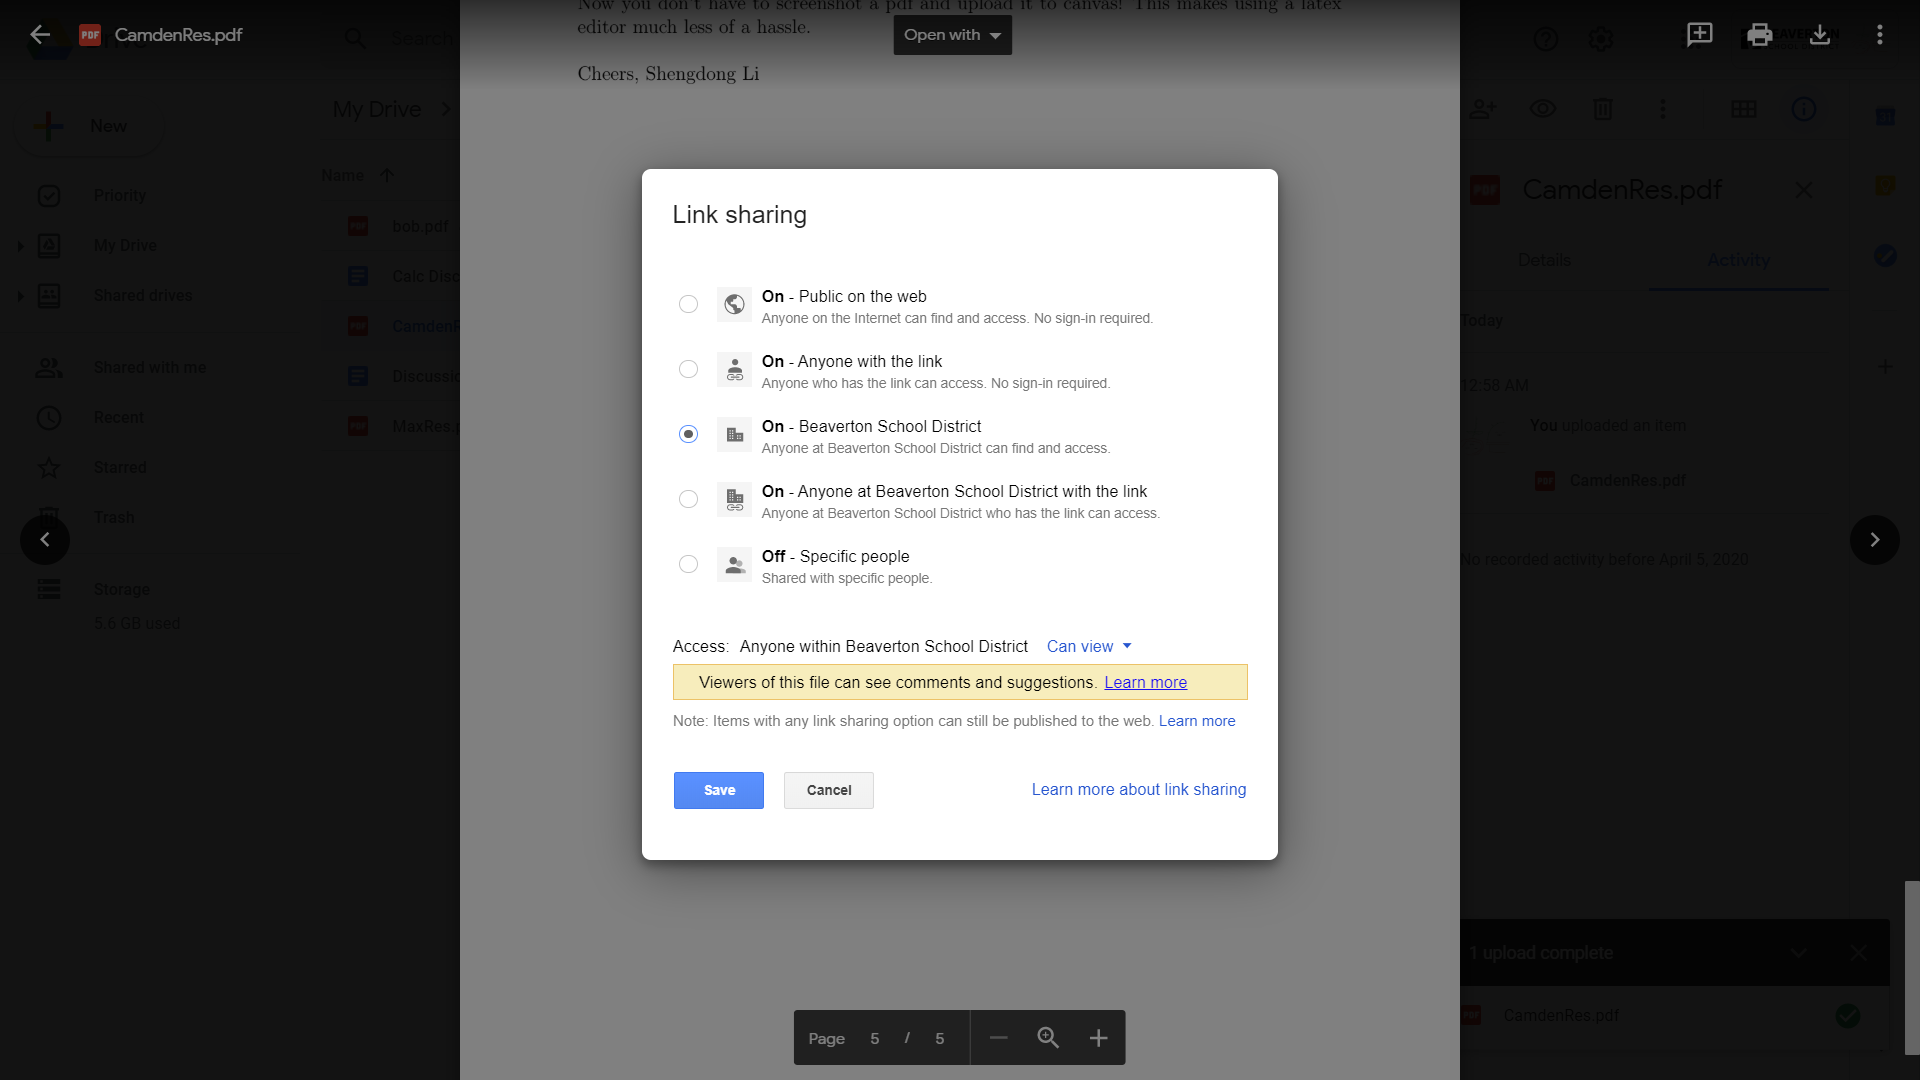
\includegraphics[scale=0.3]{9.png}
\end{center}
Now you don't have to screenshot a pdf and upload it to canvas! This makes using a latex editor much less of a hassle.\\~\\
Cheers, Shengdong Li
\end{document}